\documentclass[journel,12pt,twocoloums]{IEEEtran}

\title{Assignment 3 -Probability and Random Variable}
\author{Annu-EE21RESCH01010}
\date{13 January 2020}
\usepackage{tikz}
\usetikzlibrary{automata, positioning}
\usepackage{amsthm}
\usepackage{graphicx}
\usepackage{mathrsfs}
\usepackage{txfonts}
\usepackage{stfloats}
\usepackage{pgfplots}
\usepackage{cite}
\usepackage{cases}
\usepackage{mathtools}
\usepackage{caption}
\usepackage{enumerate}	
\usepackage{enumitem}
\usepackage{amsmath}
\usepackage[utf8]{inputenc}
\usepackage[english]{babel}
\usepackage{multicol}
%\usepackage{xtab}
\usepackage{longtable}
\usepackage{multirow}
%\usepackage{algorithm}
%\usepackage{algpseudocode}
\usepackage{enumitem}
\usepackage{mathtools}
\usepackage{gensymb}
\usepackage{hyperref}
%\usepackage[framemethod=tikz]{mdframed}
\usepackage{listings}
    %\usepackage[latin1]{inputenc}                                 %%
    \usepackage{color}                                            %%
    \usepackage{array}                                            %%
    \usepackage{longtable}                                        %%
    \usepackage{calc}                                             %%
    \usepackage{multirow}                                         %%
    \usepackage{hhline}                                           %%
    \usepackage{ifthen}                                         %%
  \providecommand{\nCr}[2]{\,^{#1}C_{#2}}
  \providecommand{\nPr}[2]{\,^{#1}P_{#2}}
  \lstset{
%language=C,
frame=single, 
breaklines=true,
columns=fullflexible
}

 \begin{document}
 \maketitle
 \textbf{Download Python code from here}\\
\begin{lstlisting}
 https://github.com/annu100/AI5002-Probability-and-Random-variables/blob/main/ASSIGNMENT_3/Assignment_3_Bayes.py
 \end{lstlisting}
\textbf{Download latex code from here-}\\
\begin{lstlisting}
 https://github.com/annu100/AI5002-Probability-and-Random-variables/blob/main/ASSIGNMENT_3/main.tex
 \end{lstlisting}
 \section{Problem Statement-Problem 2.10}
Bag I contains 3 red and 4 black balls and
Bag II contains 4 red and 5 black balls. One
ball is transferred from Bag I to Bag II and
then a ball is drawn from Bag II. The ball
so drawn is found to be red in colour. Find
the probability that the transferred ball is black.
\\
\\
\section{Solutions}
Bag 1 contains 3 red and 4 black balls.\\
Bag 2 contains 4 red and 5 black balls.\\

let  C1: Event of transferring black ball from bag 1 to 2\\
let  C1: Event of transferring red ball from bag 1 to 2\\
let A : Event that the ball drawn from 2 is red after the transfer of a ball from bag 1 to bag 2.\\
\\
\\
\\
\\
\\
\\
\\

\textbf{Using markov chain} \\
\begin{tikzpicture}[font=\sffamily]

        % Setup the style for the states
        \tikzset{node style/.style={state, 
                                    minimum width=2cm,
                                    line width=1mm,
                                    fill=gray!20!white}}

       % Draw the states
        \node[node style] at (0, 0)     (C1)     {C1};
        \node[node style] at (6, 0)     (C2)     {C2};
        \node[node style] at (3, -5.196) (A) {A};

        % Connect the states with arrows
        \draw[every loop,
              auto=right,
              line width=1mm,
              >=latex,
              draw=orange,
              fill=orange]
            (C1)     edge[bend right=20]            node {$\frac{2}{5}$} (A)
            (C1)     edge[loop above]            node {$\frac{4}{7}$} (C1)
            (C2)     edge[loop above]            node {$\frac{3}{7}$} (C2)
            (C2)     edge[bend right=20, auto=left] node {$\frac{1}{2}$} (A)
            (A) edge[bend right=20]            node {$\frac{15}{31}$} (C2)
            (A) edge[bend right=20, auto=left] node {$\frac{16}{31}$} (C1);
    \end{tikzpicture}
 Note that:Above drawn markov chain is 3 states first order time homogeneous markov chain as transition probabilities are depending only on last one state.\\
 $Pr(A|C1)$:Representing transition probability for going state A from state C1.\\
 $Pr(A|C2)$:Representing transition probability for going state A from state C2.\\
 Pr(C1):Representing  probability to remain in C1.\\
 Pr(C2):Representing  probability to remain in C2.\\
\begin{align*}
Pr(C1)= \frac{4}{7}\\
Pr(C2)=\frac{3}{7}\\
Pr(A|C1)=\frac{4}{10}=\frac{2}{5}\\
Pr(A|C2)=\frac{5}{10}=\frac{1}{2}\\
\text{From Baye's theoram} \\
Pr(\text{Drawn ball is red})&=P(A)\\
                     &=Pr(\frac{A}{C1})\times Pr(C1)\\
                     &    +Pr(C2)\times Pr(\frac{A}{C2})\\
                     &=\frac{4}{10}\times \frac{4}{7}+\frac{5}{10}\times \frac{3}{7}\\
                     &=\frac{16+15}{70}\\
                     &=\frac{31}{70}
\end{align*}


The probability that the transferred ball is black\\
It is equal to conditional probability of C1 when event A has already happened\\
Calculating probabilities for markov chain.\\
\begin{align*}
Pr(\frac{C1}{A})&=\frac{Pr(C1 \cap A)}{Pr(A)}\\
        &=\frac{Pr(\frac{A}{C1})Pr(C1)}{Pr(A)}\\
        &=\frac{\frac{4}{10} \times \frac{4}{7}}{\frac{31}{70}}\\
        &=\frac{16}{31}
\end{align*}
\begin{align*}
Pr(\frac{C2}{A})&=\frac{Pr(C2 \cap A)}{Pr(A)}\\
        &=\frac{Pr(\frac{A}{C2})Pr(C2)}{Pr(A)}\\
        &=\frac{\frac{5}{10} \times \frac{3}{7}}{\frac{31}{70}}\\
        &=\frac{15}{31}
\end{align*}

We have been asked to find out $Pr(C|A)$
Hence the desired probability is $$\frac{16}{31}=0.516$$\\
\\

\section{simulation part}

Using random variable simulation,bernaulli random variables are generated for the two cases:-
P(X=0)=probability for drawnball
P(X=1)=probability for transffered ball \\
\\
\\

\begin{figure}[!htb]
    \centering
    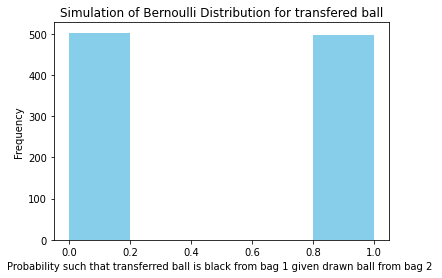
\includegraphics[width=\columnwidth]{simulation.png}
    \caption{simulation of bernaulli distribution for transferred ball}
    \label{fig:frequency vs n}
\end{figure}

\end{document}
      

